\documentclass[12pt]{article} % use larger type; default would be 10pt
\usepackage[czech]{babel}
\usepackage[utf8]{inputenc} % set input encoding (not needed with XeLaTeX)

%%% PAGE DIMENSIONS
\usepackage{geometry} % to change the page dimensions
% \usepackage[left=2cm,right=2cm,top=2cm,bottom=2cm]{geometry}
\geometry{a4paper}
% \geometry{margin=2in} % for example, change the margins to 2 inches all round
% \geometry{landscape} % set up the page for landscape

\usepackage{graphicx} % support the \includegraphics command and options
\usepackage{wrapfig} % support the wrapfigure section

\usepackage{hyperref} % links in \tableofcontents
\hypersetup{
	colorlinks,
	citecolor=black,
	filecolor=black,
	linkcolor=black,
	urlcolor=black
}

% \usepackage[parfill]{parskip} % Activate to begin paragraphs with an empty line rather than an indent

%%% PACKAGES
\usepackage{booktabs} % for much better looking tables
\usepackage{array} % for better arrays (eg matrices) in maths
%\usepackage{paralist} % very flexible & customisable lists (eg. enumerate/itemize, etc.)
\usepackage{verbatim} % adds environment for commenting out blocks of text & for better verbatim
\usepackage{subfig} % make it possible to include more than one captioned figure/table in a single float
% These packages are all incorporated in the memoir class to one degree or another...
\usepackage{tikz} % graphs
\usepackage{pgfplots}
\usepackage{float}

%%% HEADERS & FOOTERS
\usepackage{fancyhdr} % This should be set AFTER setting up the page geometry
\pagestyle{fancy} % options: empty , plain , fancy
\renewcommand{\headrulewidth}{0pt} % customise the layout...
\lhead{}\chead{}\rhead{}
\lfoot{}\cfoot{\thepage}\rfoot{}

%%% SECTION TITLE APPEARANCE
\usepackage{sectsty}
\allsectionsfont{\sffamily\mdseries\upshape} % (See the fntguide.pdf for font help)
% (This matches ConTeXt defaults)

%%% ToC (table of contents) APPEARANCE
\usepackage[nottoc,notlof,notlot]{tocbibind} % Put the bibliography in the ToC
\usepackage[titles,subfigure]{tocloft} % Alter the style of the Table of Contents
\renewcommand{\cftsecfont}{\rmfamily\mdseries\upshape}
\renewcommand{\cftsecpagefont}{\rmfamily\mdseries\upshape} % No bold!
\newcommand{\bigsize}{\fontsize{35pt}{20pt}\selectfont}

%%% END Article customizations

\begin{document}
\begin{titlepage}
	
\includegraphics[scale=0.7]{logo.jpg}
	\vspace*{\fill}
	\begin{center}
		\textsc{\LARGE Katedra technologií a měření}\\[0.3cm]
		\textsc{\LARGE \bigsize Fyzikální elektronika}\\[0.3cm]
		\textsc{\LARGE Unipolární tranzistory}\\[1cm]
		Martin Zlámal \\
		Josef Sedlák \\[1cm]
		{\small\em \ Datum měření 2. prosince 2013 } \\
		{\small\em \copyright \ Datum poslední revize \today } \\
		\LaTeX
	\end{center}
	\vspace*{\fill}
\end{titlepage}
\tableofcontents
\listoffigures
\listoftables
\newpage

\section{Schéma zapojení}
\begin{figure}[H]
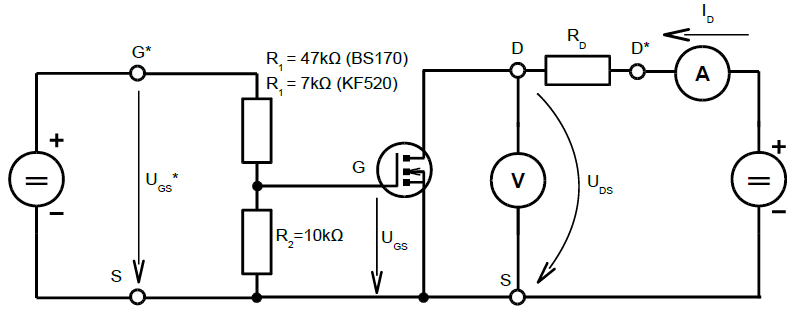
\includegraphics[scale=0.7]{schema.png}
\caption{Schéma zapojení úlohy}
\end{figure}

\section{Katalogové parametry měřených součástek}
\begin{table}[H]
\caption{Katalogové parametry měřených součástek}
\begin{tabular}{|c|c|c|}
\hline 
Typ tranzistoru & BS170 & KF520 \\ 
\hline 
$I_D\,[mA]$ & $500$ & $30$ \\ 
\hline 
$U_{DS}\,[V]$ & $60$ & $30$ \\ 
\hline 
$P_{TOT}\,[mW]$ & $350$ & $300$ \\ 
\hline 
\end{tabular} 
\end{table}

\section{Naměřené a vypočtené hodnoty}
\begin{table}[H]
\caption{Data výstupní charakteristiky tranzistoru KF520}
\begin{tabular}{|c|c||c|c||c|c||c|c|}
\hline 
\multicolumn{2}{|c|}{$U_{GS}^*=0\,V$} & \multicolumn{2}{|c|}{$U_{GS}^*=3\,V$} & \multicolumn{2}{|c|}{$U_{GS}^*=6\,V$} & \multicolumn{2}{|c|}{$U_{GS}^*=-3\,V$} \\ 
\hline 
\multicolumn{2}{|c|}{$U_{GS}=0\,V$} & \multicolumn{2}{|c|}{$U_{GS}=1,76\,V$} & \multicolumn{2}{|c|}{$U_{GS}=3,53\,V$} & \multicolumn{2}{|c|}{$U_{GS}=-1,76\,V$} \\ 
\hline 
$U_{DS}\,[V]$ & $I_D\,[mA]$ & $U_{DS}\,[V]$ & $I_D\,[mA]$ & $U_{DS}\,[V]$ & $I_D\,[mA]$ & $U_{DS}\,[V]$ & $I_D\,[mA]$ \\ 
\hline 
0 & 0 & 0 & 0 & 0 & 0 & 0 & 0 \\ 
\hline 
0,22 & 0,17 & 0,32 & 0,29 & 0,15 & 0,16 & 0,36 & 0,23 \\ 
\hline 
0,35 & 0,26 & 0,57 & 0,5 & 0,3 & 0,32 & 0,67 & 0,39 \\ 
\hline 
0,43 & 0,32 & 0,93 & 0,77 & 0,64 & 0,64 & 1,11 & 0,56 \\ 
\hline 
0,61 & 0,44 & 1,24 & 0,98 & 1,0 & 0,97 & 1,45 & 0,67 \\ 
\hline 
0,80 & 0,56 & 1,52 & 1,14 & 1,27 & 1,18 & 1,76 & 0,75 \\ 
\hline 
0,95 & 0,64 & 1,78 & 1,29 & 1,61 & 1,43 & 2,08 & 0,81 \\ 
\hline 
1,26 & 0,8 & 2,14 & 1,47 & 1,9 & 1,63 & 2,36 & 0,86 \\ 
\hline 
1,38 & 0,86 & 2,89 & 1,75 & 2,23 & 1,83 & 2,69 & 0,9 \\ 
\hline 
1,56 & 0,94 & 3,51 & 1,93 & 2,52 & 1,99 & 3,07 & 0,92 \\ 
\hline 
1,76 & 1,02 & 4,0 & 2,03 & 3,25 & 2,33 & 3,58 & 0,95 \\ 
\hline 
2,02 & 1,11 & 4,78 & 2,13 & 4,36 & 2,69 & 4,42 & 0,96 \\ 
\hline 
2,34 & 1,21 & 6,82 & 2,23 & 5,55 & 2,91 & 5,23 & 0,97 \\ 
\hline 
2,64 & 1,28 & 8,31 & 2,25 & 6,74 & 3,02 & 7,23 & 0,98 \\ 
\hline 
3,0 & 1,35 & 10,2 & 2,28 & 7,94 & 3,06 & 9,66 & 0,99 \\ 
\hline 
6,91 & 1,54 & 15,24 & 2,31 & 10,77 & 3,12 & 14,33 & 1,01 \\ 
\hline 
8,01 & 1,56 & 19,06 & 2,34 & 13,1 & 3,14 & 17,74 & 1,02 \\ 
\hline 
\end{tabular} 
\end{table}

Hodnota napětí $U_{GS}^*$ značí napětí na odporovém děliči. Napětí přímo na řídící elektrodě transistoru dopočteme $U_{GS}$ dopočteme jako:
\begin{equation}
U_{GS} = U_{GS}^* \cdot \frac{R_2}{R_1+R_2} = 3 \cdot \frac{10}{7+10} = 1,76\,V
\end{equation}
Pro vypočtení napětí na řídící elektrodě pro tranzistor BS170 použijeme stejný postup, jen hodnota $R_1 = 47\,k\Omega$.

Hodnoty převodní impedance $y_{21}$ pro oba tranzistory:
\begin{equation}
y_{21}(KF520) = \frac{\Delta I_D}{\Delta U_{GS}} = \frac{3,06-1,56}{3,53-0} = 0,425\,mS
\end{equation}
\begin{equation}
y_{21}(BS170) = \frac{\Delta I_D}{\Delta U_{GS}} = \frac{9,75-9,34}{2,39-2,19} = 2,05\,mS
\end{equation}

\begin{table}
\caption{Data výstupní charakteristiky tranzistoru BS170}
\begin{tabular}{|c|c|c|c|c|c|c|c|}
\hline 
\multicolumn{2}{|c|}{$U_{GS}^*=12,5\,V$} & \multicolumn{2}{|c|}{$U_{GS}^*=13,0\,V$} & \multicolumn{2}{|c|}{$U_{GS}^*=13,3\,V$} & \multicolumn{2}{|c|}{$U_{GS}^*=13,6\,V$} \\ 
\hline 
\multicolumn{2}{|c|}{$U_{GS}=2,19\,V$} & \multicolumn{2}{|c|}{$U_{GS}=2,28\,V$} & \multicolumn{2}{|c|}{$U_{GS}=2,33\,V$} & \multicolumn{2}{|c|}{$U_{GS}=2,39\,V$} \\ 
\hline 
$U_{DS}\,[V]$ & $I_D\,[mA]$ & $U_{DS}\,[V]$ & $I_D\,[mA]$ & $U_{DS}\,[V]$ & $I_D\,[mA]$ & $U_{DS}\,[V]$ & $I_D\,[mA]$ \\ 
\hline 
0 & 0 & 0 & 0 & 0 & 0 & 0 & 0 \\ 
\hline 
0,03 & 0,6 & 0,03 & 1,06 & 0,02 & 1,09 & 0,02 & 1,39 \\ 
\hline 
0,06 & 0,92 & 0,06 & 1,73 & 0,04 & 1,86 & 0,04 & 2,5 \\ 
\hline 
0,08 & 0,99 & 0,08 & 2,09 & 0,06 & 2,43 & 0,06 & 3,44 \\ 
\hline 
0,1 & 1,17 & 0,1 & 2,43 & 0,08 & 2,9 & 0,08 & 4,2 \\ 
\hline 
0,15 & 1,2 & 0,15 & 2,48 & 0,1 & 3,54 & 0,1 & 5,2 \\ 
\hline 
0,2 & 1,35 & 0,2 & 2,87 & 0,2 & 4,33 & 0,2 & 6,06 \\ 
\hline 
0,3 & 1,41 & 0,3 & 3,05 & 0,3 & 4,56 & 0,3 & 6,55 \\ 
\hline 
0,4 & 1,44 & 0,4 & 3,11 & 0,4 & 4,68 & 0,4 & 6,76 \\ 
\hline 
0,5 & 1,45 & 0,5 & 3,16 & 0,5 & 4,72 & 0,5 & 6,87 \\ 
\hline 
2 & 1,56 & 2,0 & 3,36 & 2, & 5,05 & 1,26 & 7,18 \\ 
\hline 
3 & 1,59 & 3,1 & 3,46 & 3,27 & 5,2 & 2,24 & 7,42 \\ 
\hline 
4 & 1,63 & 4,23 & 3,56 & 4,25 & 5,35 & 3,36 & 7,65 \\ 
\hline 
5,5 & 1,69 & 4,92 & 3,62 & 5,0 & 5,48 & 5,42 & 8,12 \\ 
\hline 
6,89 & 1,72 & 5,72 & 3,7 & 6,3 & 5,69 & 8,5 & 8,95 \\ 
\hline 
8,42 & 1,82 & 7,26 & 3,87 & 8,05 & 6,0 & 10,63 & 9,75 \\ 
\hline 
10,7 & 1,95 & 9,34 & 4,02 & 10,42 & 6,55 & 14,3 & 11,9 \\ 
\hline 
15 & 2,23 & 14,71 & 4,89 & 14,72 & 7,63 &   &   \\ 
\hline 
\end{tabular} 
\end{table}

\begin{table}
\caption{Data převodní charakteristiky tranzistoru BS170}
\begin{tabular}{|c|c|c||c|c|c|}
\hline 
\multicolumn{3}{|c|}{$U_{DS}=5\,V$} & \multicolumn{3}{|c|}{$U_{DS}=10\,V$} \\ 
\hline 
$U_{GS}^*\,[V]$ & $U_{GS}\,[V]$ & $I_D\,[mA]$ & $U_{GS}^*\,[V]$ & $U_{GS}\,[V]$ & $I_D\,[mA]$ \\ 
\hline 
10,0 & 1,75 & 0,0073 & 10,0 & 1,75 & 0,0085 \\ 
\hline 
10,5 & 1,84 & 0,0238 & 10,5 & 1,84 & 0,0291 \\ 
\hline 
11,0 & 1,93 & 0,0684 & 11,0 & 1,93 & 0,0799 \\ 
\hline 
11,5 & 2,02 & 0,247 & 11,5 & 2,02 & 0,243 \\ 
\hline 
12,0 & 2,11 & 0,629 & 12,0 & 2,11 & 0,72 \\ 
\hline 
12,5 & 2,19 & 1,667 & 12,5 & 2,19 & 1,9 \\ 
\hline 
13,0 & 2,28 & 3,66 & 13,0 & 2,28 & 3,82 \\ 
\hline 
13,5 & 2,37 & 7,05 & 13,5 & 2,37 & 8,73 \\ 
\hline 
14,0 & 2,46 & 13,04 & 14,0 & 2,46 & 15,86 \\ 
\hline 
\end{tabular} 
\end{table}

\section{Grafy}
\begin{figure}[H]
\center
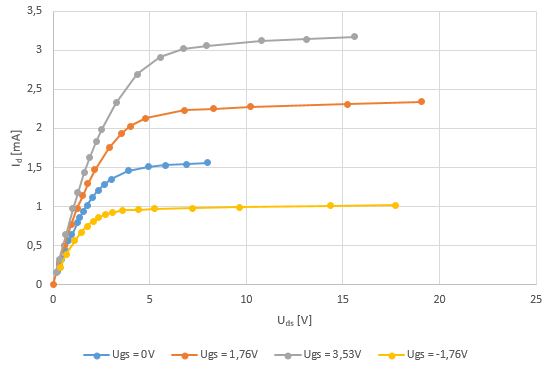
\includegraphics[scale=0.9]{vystup_kf520.png}
\caption{Výstupní charakteristika tranzistoru KF520}
\end{figure}

\begin{figure}[H]
\center
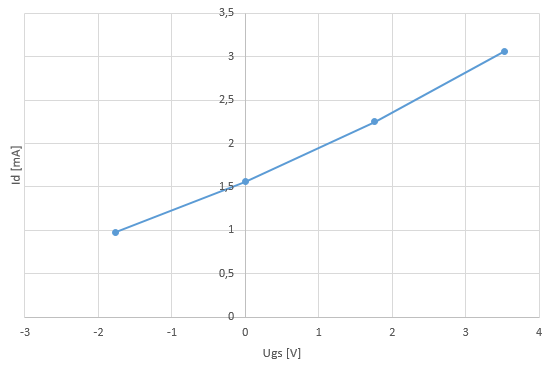
\includegraphics[scale=0.8]{prevodni_kf520.png}
\caption{Odvozená převodní charakteristika tranzistoru KF520}
\end{figure}

\begin{figure}[H]
\center
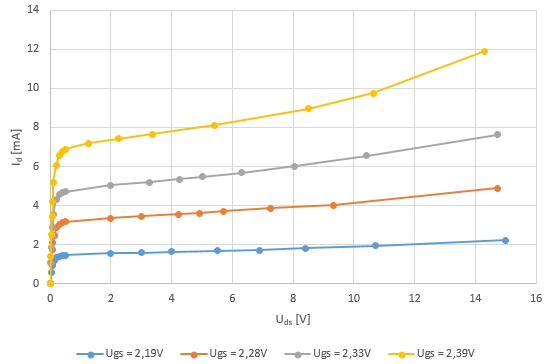
\includegraphics[scale=0.9]{vystup_bs170.png}
\caption{Výstupní charakteristika tranzistoru BS170}
\end{figure}

\begin{figure}[H]
\center
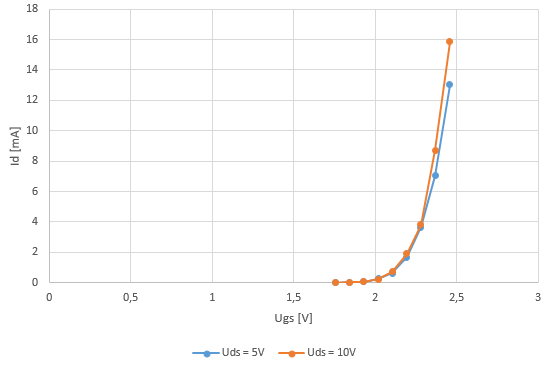
\includegraphics[scale=0.9]{prevodni_bs170.png}
\caption{Převodní charakteristika tranzistoru BS170}
\end{figure}

\begin{figure}[H]
\center
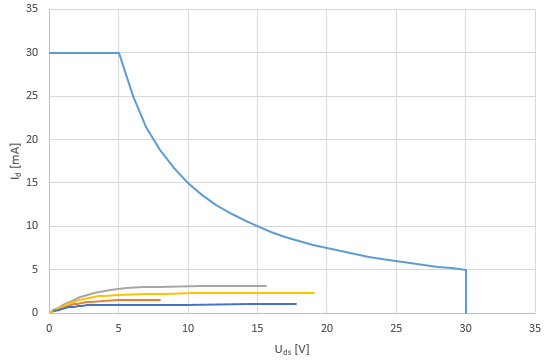
\includegraphics[scale=0.9]{mezni_kf520.png}
\caption{Vizualizované mezní parametry tranzistoru KF520}
\end{figure}

\begin{figure}[H]
\center
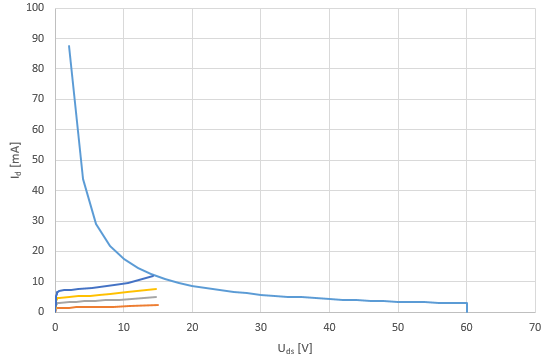
\includegraphics[scale=0.9]{mezni_bs170.png}
\caption{Vizualizované mezní parametry tranzistoru BS170}
\end{figure}

\section{Závěr}
Se vzrůstajícím napětím na řídící elektrodě $U_{GS}$ vzrůstá také samotná křivka výstupní charakteristiky unipolárních transistorů. Toto napětí může nabývat u tranzistoru KF520 záporných hodnot, u tranzistoru BS170 již to není možné. Toto je vidět také z převodních charakteristik. Tam kde lze dosáhnout záporných hodnot na řídící elektrodě přesahuje graf do záporného kvadrantu. Oproti tomu u tranzistoru BS170 tomu tak není a převodní charakteristika má exponenciální tvar. Z této charakteristiky je také vidět, že existuje jistá minimální hranice řídícího napětí $U_{GS}$, pod kterou již je tranzistor prakticky nepoužitelný, protože by se na výstupní charakteristice nic neprojevilo.

\end{document}